\documentclass[../sparc.tex]{subfiles}
\graphicspath{{\subfix{../images/}}}
\begin{document}

%%%%%%%%%%%%%%%%%%%%%%%%%%%%%%%%%%%%%%%%%%%%%%%%%%%%%%%%%%%%%%%%%%%%%%%%%%%%%%%%
\section{Electric Circuits}
\index{Electronics!Electric Circuits}

Now let's imagine two vessels, one of which holds ten liters of water and the
second one holds zero liters (or, as people usually say, it is \emph{empty}), as
shown on the fig. \ref{fig:electronics-circuits-0}.

\begin{figure}[ht]
  \centering
  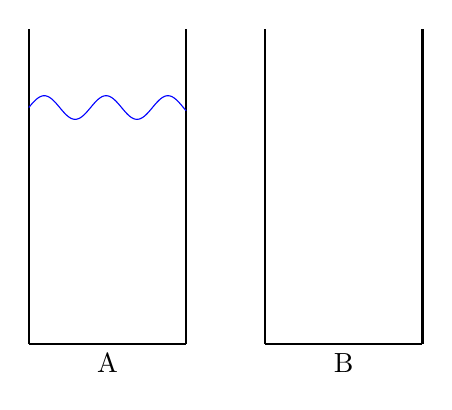
\begin{tikzpicture}[
      declare function={f1(\x) = 0.15 * sin(8.0 * deg(\x));
    }]

    \draw[thick] (0, 0) -- (0, 4);
    \draw[thick] (2, 0) -- (2, 4);
    \draw[thick] (0, 0) -- (2, 0);

    \draw[thick] (3, 0) -- (3, 4);
    \draw[thick] (5, 0) -- (5, 4);
    \draw[thick] (3, 0) -- (5, 0);

    \begin{scope}[yshift=3cm, color=blue]
      \draw (0, 0) plot[domain=0:2, variable=\x, samples=200, smooth] ({\x}, {f1(\x)});
    \end{scope}

    \draw (1, 0) node[below] {A};
    \draw (4, 0) node[below] {B};

  \end{tikzpicture}
  \caption{An example of two vessels: one filled with water (A) and one that is
    empty (B).}
  \label{fig:electronics-circuits-0}
\end{figure}

If we connect the vessel ``A'' with the vessel ``B'' the water will flow from
``A'' to ``B'' due to the laws of physics (as shown in fig.
\ref{fig:electronics-circuits-1}.)

\begin{figure}[ht]
  \centering
  \begin{tikzpicture}[
      declare function={f1(\x) = 0.15 * sin(8.0 * deg(\x));
    }]

    \draw[thick] (0, 0) -- (0, 4);
    \draw[thick] (2, 0.5) -- (2, 4);
    \draw[thick] (0, 0) -- (2, 0);

    \draw[thick] (3, 0.5) -- (3, 4);
    \draw[thick] (5, 0) -- (5, 4);
    \draw[thick] (3, 0) -- (5, 0);

    \draw[thick] (2, 0) -- (3, 0);
    \draw[thick] (2, 0.5) -- (3, 0.5);

    \draw[thick, color=blue, -{Implies}, double] (2, 0.25) -- (3, 0.25);

    \begin{scope}[yshift=3cm, color=blue]
      \draw (0, 0) plot[domain=0:2, variable=\x, samples=200, smooth] ({\x}, {f1(\x)});
    \end{scope}
    \draw[thick, color=blue, -{Implies}, double] (1, 3cm) -- (1, 2cm);

    \begin{scope}[yshift=0.75cm, xshift=3cm, color=blue]
      \draw (0, 0) plot[domain=0:2, variable=\x, samples=200, smooth] ({\x}, {f1(\x)});
    \end{scope}
    \draw[thick, color=blue, -{Implies}, double] (4, 1cm) -- (4, 2cm);

    \draw (1, 0) node[below] {A};
    \draw (4, 0) node[below] {B};

  \end{tikzpicture}
  \caption{An example of two vessels with different levels of water connected
    with a pipe.}
  \label{fig:electronics-circuits-1}
\end{figure}

When we connected vessels ``A'' and ``B'' with a pipe we've got a \emph{closed
circuit} that allows the flow of water.  Electrical circuits work in the similar
way, but instead of the water flow they conduct the flow of elementary charged
particles.

Thus here goes the second rule that we need to learn: electrical current is
possible only in closed circuits.

Electrical current is measured in \emph{Amperes} (A).

Figure \ref{fig:electronics-simple-circuit} shows an electrical circuit that is
analogous to the one pictured on fig. \ref{fig:electronics-circuits-1}.

%% TODO: Re-draw the example water piping as it does not have a "functional
%% component".

\begin{figure}[ht]
  \centering
  \begin{circuitikz}
    \draw (0,0)
    to[battery, l=Battery] (0,2) % The voltage source
    to[short] (2,2)
    to[full led, l=LED] (2,0) % The lamp
    to[short] (0,0);
  \end{circuitikz}
  \caption{An electrical circuit that uses a battery as the power source and a
    LED as a functional component.}
  \label{fig:electronics-simple-circuit}
\end{figure}

\end{document}
